\documentclass[]{scrartcl}

\usepackage{labrep}

%opening
\title{Resonance in series and parallel circuit}
\author{Grzegorz Potocki}
\date{20 November 2023}

\begin{document}
	
\begin{center}
	\makeatletter
	\renewcommand{\arraystretch}{2.0}% for the vertical padding

\begin{tabular}{|M{\linewidth}|}
	\hline
	
	{\LARGE Poznan University of Technology}\\
	{\LARGE Institute of Electrical Engineering and Electronics}\\
	{\LARGE Electrical and Electronics Engineering Project}\\ \hline
    \multicolumn{1}{|l|}{Title: \@title }\\ \hline
	\multicolumn{1}{|l|}{Author: \@author} \\ \hline
	\multicolumn{1}{|l|}{Date: \@date} \\
	\hline
	
\end{tabular}
\makeatother
\vspace{1.5cm}
\end{center}

\section{Introduction}

\begin{flushleft}
    Resonance in RLC circuits occurs when the so-called resonant frequency is applied to the circuit. It is a specific frequency which causes the cancellation of admittance and impedance. This phenomena behaves different in series and parallel circuits.
\end{flushleft}  

\begin{flushleft}
    The series resonance also called the voltage resonance occurs when  the inductive reactance $X_L$ and capacitive reactance $X_C$ are equal in magnitude but opposite in phase (simply when reactance of whole circuit is equal to zero $X=X_L+X_C=0$). This condition results in the cancellation of these reactances, leaving only the resistance $R$ in the circuit. 
\end{flushleft}

\begin{flushleft}
    The parallel resonance also called the current resonance or anti-resonance occurs when inductive susceptance $B_L$ and capacitive susceptance $B_C$ are equal in magnitude but opposite in phase (simply when susceptance of whole circuit is equal to zero $B=B_L+B_C=0$). This condition results in large circulating current between the inductor and the capacitor
\end{flushleft}

\section{The process of the exercise}

\subsection{Determine the frequency of the generator for which there is a maximum voltage drop at the resistance, and the voltage on capacitor and inductor will be the same}

\subsubsection{Scheme}

\begin{figure}[H]
	\centering
	\begin{circuitikz}[american voltages, american currents, european resistors]
    \node[draw,minimum width=1.2cm,minimum height=2cm,anchor=south west] at (0,0){};
    \draw
    (-1, 1.5) [short, o-] to (0, 1.5) node [anchor=west] {G};
    \draw
    (-1, 0.5) [short, o-] to (0, 0.5);
    \draw
    (1.2, 0.6) node [anchor=east] {f} [short] to (1.4, 0.3) 
    to [short] (1.4, -0.4)
    (1.2, -0.4) to [short] (1.6, -0.4);
    \draw
    (1.2, 1.4) to (1.8, 1.4)
    to [short] (1.8, 2.4)
    to [short] (3, 2.4)
    to [C,l_=$C$] (6, 2.4)
    to [L,l_=$L$] (9, 2.4)
    to [short] (11, 2.4)
    to [rmeterwa, t=$V_R$] (11, -0.4)
    to [short] (1.8, -0.4)
    to [short] (1.8, 0.6)
    to [short] (1.2, 0.6)
    (9, 2.4) to [R=$R$,*-*] (9, -0.4)
    (3, 2.4) to [rmeterwa, t=$V_G$, *-*] (3, -0.4)
    (3.5, 2.4) to [short, *-] (3.5, 3.5)
    to [rmeterwa, t=$V_C$] (5.5, 3.5)
    to [short, -*] (5.5, 2.4)
    (6.5, 2.4) to [short, *-] (6.5, 3.5)
    to [rmeterwa, t=$V_L$] (8.5, 3.5)
    to [short, -*] (8.5, 2.4);
\end{circuitikz}
	\caption{Series RLC circuit for measuring resonance}
	\label{fig:circuitfig_series}
\end{figure}

Data: U=2[V], R=1000[$\Omega$], L=56[mH], C=5060[pF] 

\subsubsection{Measurement process}

First part of the exercise aims to correctly assemble the circuit according to diagram 6.2.2.1 and connect the voltmeters to all RLC elements in the circuit in order to measure their voltages at the same time. Next task is to find the frequency of the generator at constant voltage 2V when voltage of the capacitor and inductor is the same(hence there is a maxiumum voltage drop at the resistor).

\begin{table}[hptb]
	\centering
	\caption{Measurements of series circuit}
	\label{tab:tab1}
	\begin{tabular}{|c|c|c|c|c|}
		\hline
		No. & Frequency [\unit{\hertz}] & $U_R$ [\unit{\volt}] & $U_L$ [\unit{\volt}] & $U_C$ [\unit{\volt}] \\   
		\hline
		1& 10800 & 1.35 & 5.25 & 4.02\\
		\hline
		2& 10600 & 1.44 & 5.49 & 4.36\\
		\hline
		3& 10400 & 1.53 & 5.70 & 4.705\\
		\hline
		4& 10200 & 1.62 & 5.92 & 4.867\\
		\hline
        5& 10000 & 1.709 & 6.117 & 5.244\\
		\hline
        6& 9800 & 1.787 & 6.264 & 5.609\\
		\hline
        7& 9600 & 1.8465 & 6.332 & 5.915\\
		\hline
        8& 9475 & 1.87 & 6.326 & 6.077\\
		\hline
        9& 9375 & 1.88 & 6.288 & 6.175\\
		\hline
        10& 9325 & 1.882 & 6.258 & 6.21\\
		\hline
        11& 9300 & 1.881 & 6.23 & 6.22\\
		\hline
        12& 9275 & 1.8812 & 6.217 & 6.24\\
		\hline
        13& 9225 & 1.878 & 6.17 & 6.27\\
		\hline
        14& 9125 & 1.866 & 6.06 & 6.397\\
		\hline
        15& 9000 & 1.84 & 5.88 & 6.295\\
		\hline
        16& 8800 & 1.77 & 5.526 & 6.195\\
		\hline
        17& 8600 & 1.677 & 5.107 & 6.009\\
		\hline
        18& 8400 & 1.574 & 4.66 & 5.76\\
		\hline
        19& 8200 & 1.459 & 4.304 & 5.48\\
		\hline
        20& 8000 & 1.348 & 3.876 & 5.19\\
		\hline
        21& 7800 & 1.2426 & 3.48 & 4.90\\
		\hline
	\end{tabular}
\end{table}

\subsection{Make voltage measurements on the resistance, coil and capacitor at frequencies taken from Table, maintaining a constant value of the generator voltage (5 V)}

\subsubsection{Scheme}

\begin{figure}[H]
	\centering
	\begin{circuitikz}[american voltages, american currents, european resistors]
    \node[draw,minimum width=1.2cm,minimum height=2cm,anchor=south west] at (0,0){};
    \draw
    (-1, 1.5)  [short, o-] to (0, 1.5) node [anchor=west] {G};
    \draw
    (-1, 0.5) [short, o-] to (0, 0.5);
    \draw
    (1.2, 0.6) node [anchor=east] {f} [short] to (1.4, 0.3) 
    to [short] (1.4, -0.4)
    (1.2, -0.4) to [short] (1.6, -0.4);
    \draw
    (1.2, 1.4) to (1.8, 1.4)
    to [short] (1.8, 2.4)
    to [short] (3, 2.4)
    to [R,l_=$R$] (6, 2.4)
    to [short] (11, 2.4)
    to [rmeterwa, t=$V_{LC}$] (11, -0.4)
    to [short] (1.8, -0.4)
    to [short] (1.8, 0.6)
    to [short] (1.2, 0.6)
    (8, 2.4) to [short, *-*] (8, 2)
    (7,2) to [short] (9,2)
    to [L=$L$] (9,0)
    to [short] (7,0)
    to [C=$C$] (7,2)
    (8,0) to [short,*-*] (8, -0.4)
    (3, 2.4) to [rmeterwa, t=$V_G$, *-*] (3, -0.4)
    (3.5, 2.4) to [short, *-] (3.5, 3.5)
    to [rmeterwa, t=$V_R$] (5.5, 3.5)
    to [short, -*] (5.5, 2.4);
\end{circuitikz}
	\caption{Parallel RLC circuit for measuring resonance}
	\label{fig:circuitfig_parallel}
\end{figure}

Data: U=5[V], R=3900[$\Omega$], L=22[mH], C=52[nF]

\subsubsection{Measurement process}

Second part of the exercise is to assemble the circuit given in 7.2.1.1. section and take voltage measurements on RLC elements for frequencies from Table 7.1 while voltage of generator have constant value 5V. Then plot the  characteristics of the relationship of the effective value of the voltage on the resistance and on the coil and capacitor as a function of frequency ($U_R=f(f)$, $U_{LC}=f(f))$.

\begin{table}[hptb]
	\centering
	\caption{Measurements of parallel circuit}
	\label{tab:tab1}
	\begin{tabular}{|c|c|c|c|c|}
		\hline
		No. & f [\unit{k\hertz}] & $|U_R|$ [\unit{\volt}] & $|U_{LC}|$ [\unit{\volt}]\\   
		\hline
		1& 1.0 & 4.97 & 0.186\\
		\hline
		2& 1.5 & 4.989 & 0.2055\\
		\hline
		3& 2.0 & 4.926 & 0.43\\
		\hline
		4& 2.5 & 4.891 & 0.607\\
		\hline
        5& 3.0 & 4.833 & 0.868\\
		\hline
        6& 3.5 & 4.696 & 1.318\\
		\hline
        7& 4.0 & 4.180 & 2.203\\
		\hline
        8& 4.5 & 4.400 & 4.11\\
		\hline
        9& 5.0 & 3.095 & 3.30\\
		\hline
        10& 5.5 & 4.205 & 2.158\\
		\hline
        11& 6.0 & 4.526 & 1.586\\
		\hline
        12& 6.5 & 4.658 & 1.254\\
		\hline
        13& 7.0 & 4.722 & 1.039\\
		\hline
        14& 7.5 & 4.760 & 0.89\\
		\hline
        15& 8.0 & 4.787 & 0.78\\
		\hline
        16& 8.5 & 4.800 & 0.098\\
		\hline
        17& 9.0 & 4.810 & 0.63\\
		\hline
        18& 9.5 & 4.928 & 0.587\\
		\hline
        19& 10.0 & 4.929 & 0.540\\
		\hline
        20& 10.5 & 4.930 & 0.502\\
		\hline
        21& 11.0 & 4.937 & 0.469\\
		\hline
        22& 11.5 & 4.943 & 0.44\\
		\hline
        23& 12.0 & 4.950 & 0.415\\
		\hline
        24& 12.5 & 4.952 & 0.301\\
		\hline
        25& 13.0 & 4.950 & 0.370\\
		\hline
        26& 13.5 & 4.955 & 0.352\\
		\hline
        27& 14.0 & 4.955 & 0.335\\
		\hline
	\end{tabular}
\end{table}

There is a mistake in taken measurements because between 4.0 and 5.0 kHz there should be a step of 0.1 instead of 0.5 kHz. It also may affect the graph which is plotted basing on this measurements. 

\section{Calculations}

\subsection{Series resonance}

\subsubsection{Designate:}

\begin{itemize}
    \item[a)]resonant pulsation
    \begin{equation}
        \omega_r=\frac{1}{\sqrt{LC}}=\frac{1}{\sqrt{56*10^{-3}*5060*10^{-12}}}=\frac{1}{\sqrt{2.8336*10^{-10}}}=59406.05707\approx59406\text{[rad/s]}
    \end{equation}
\end{itemize}

\begin{itemize}
    \item[b)]resonant frequency
    \begin{equation}
        f_0=\frac{1}{2\pi\sqrt{LC}}=\frac{\omega_r}{2\pi}\approx\frac{59406}{2\pi}\approx9454.758549\approx9460\text{[kHz]}
    \end{equation}
\end{itemize}

\begin{itemize}
    \item[c)]circuit quality factor
    \begin{equation}
        Q=\frac{U_L}{U_R}=\frac{U_C}{U_R}=\frac{\omega_rL}{R}=\frac{1}{\omega_rRC}
    \end{equation}
    
    \begin{equation}
        \frac{\omega_rL}{R}=\frac{59406.05707*56*10^{-3}}{1000}=3.326739196\approx3.3
    \end{equation}
\end{itemize}

\begin{itemize}
    \item[d)]the quality factor of the coil and capacitor at resonant pulsation, based on the given circuit parameters \\
    \begin{equation}
        Q_L=\frac{\omega_rL}{R}=\frac{59406.05707*56*10^{-3}}{1000}=3.326739196\approx3.3
    \end{equation}

    \begin{equation}
        Q_C=\frac{1}{\omega_rRC}=\frac{1}{59406.05707*1000*5060*10^{-12}}=3.326739195\approx3.3
    \end{equation}
\end{itemize}

\subsubsection{Draw the $U_R$, $U_L$, $U_C$ characteristics as a function of frequency for a series system (on one graph)}

\begin{figure}[H]
	\centering
	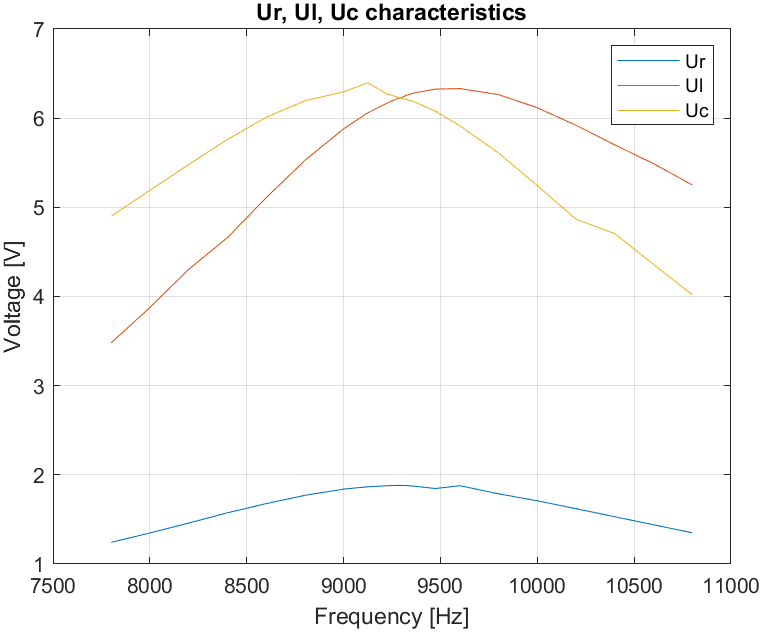
\includegraphics[width=0.7\textwidth]{Pictures/ct_char_01.png}
	\caption{$U_R$, $U_L$, $U_C$ characteristics graph}
	\label{fig:Ur, Ul, Uc char}
\end{figure}

\subsubsection{Determine the quality factor of the resonant circuit from the characteristics of
the voltage waveforms on the coil and the capacitor ($\frac{U_L}{U_0}$; $\frac{U_C}{U_0}$ as a function of frequency)}

\begin{figure}[H]
	\centering
	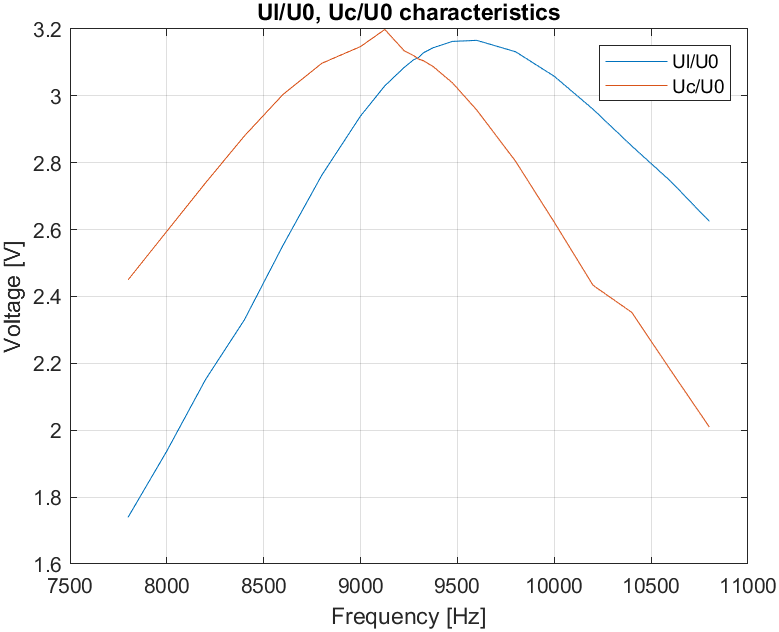
\includegraphics[width=0.7\textwidth]{Pictures/ct_char_02.png}
	\caption{$\frac{U_L}{U_0}$, $\frac{U_C}{U_0}$ characteristics graph, for this circuit $U_0=2$ [V]}
	\label{fig:Ul/U0, Uc/U0 char}
\end{figure}

\subsubsection{Cross out on one ’Characteristic line: $R$, $X_L$, $X_C$, $Z$, $X$, $X_L$-$X_C$ as a function of the relative argument}

\begin{figure}[H]
	\centering
	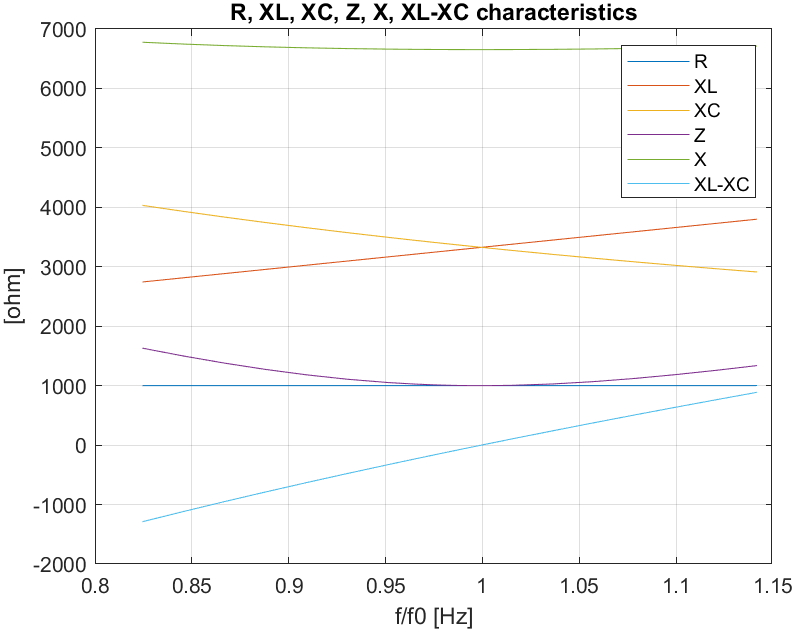
\includegraphics[width=0.7\textwidth]{Pictures/ct_char_03.png}
	\caption{$R$, $X_L$, $X_C$, $Z$, $X$, $X_L-X_C$ characteristics graph}
	\label{fig:R, XL, XC, Z, X, XL-XC char}
\end{figure}

\subsection{Parallel resonance}

\subsubsection{Plot the $|U_R|$, $|U_{LC}|$ characteristics as a function of frequency one one graph}

\begin{figure}[H]
	\centering
	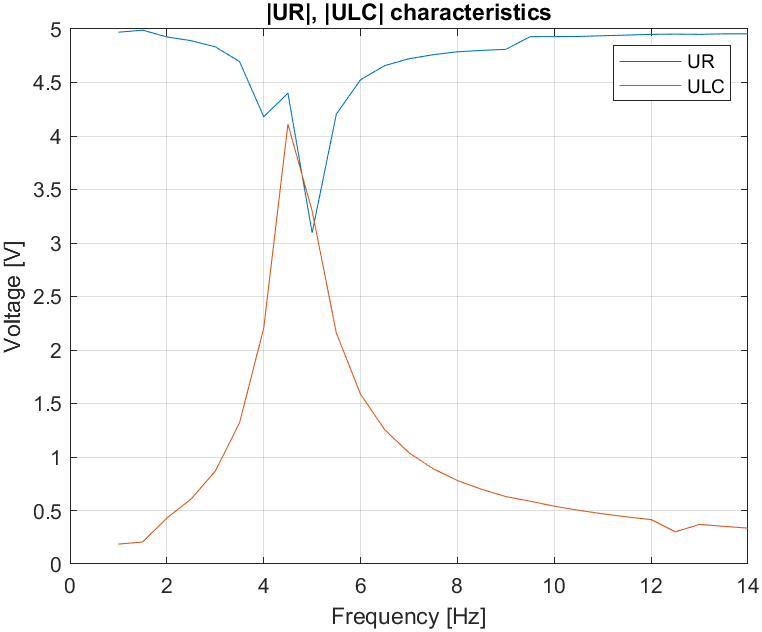
\includegraphics[width=0.7\textwidth]{Pictures/ct_char_04.png}
	\caption{$|U_R|$, $|U_{LC}|$ characteristics graph}
	\label{fig:|UR|, |ULC| char}
\end{figure}

\subsubsection{Calculate the currents flowing through the resistor, inductor and capacitor, and plot the results}

To calculate the currents flowing through resistor, inductor and capacitor it is necessary to use those formulas:

\begin{equation}
    \underline{I}_R=G\underline{U}=\frac{1}{R}\underline{U}
\end{equation}

\begin{equation}
    \underline{I}_L=-jB_L\underline{U}=-j\frac{1}{X_L}\underline{U}=-j\frac{1}{\omega L}\underline{U}
\end{equation}

\begin{equation}
    \underline{I}_C=jB_C\underline{U}=j\frac{1}{X_C}\underline{U}=j\omega C\underline{U}
\end{equation}

\begin{table}[hptb]
	\centering
	\caption{Value of currents $I_R$, $I_L$, $I_C$}
	\label{tab:tab1}
	\begin{tabular}{|c|c|c|c|c|}
		\hline
		No. & f [\unit{k\hertz}] & $I_R$ [\unit{\ampere}] & $I_L$ [\unit{\ampere}] & $I_C$ [\unit{\ampere}]\\   
		\hline
		1& 1.0 & 0.0013 & 0.00057 & 0.000026\\
		\hline
		2& 1.5 & 0.0013 & 0.00042 & 0.000043\\
		\hline
		3& 2.0 & 0.0013 & 0.00066 & 0.00019\\
		\hline
		4& 2.5 & 0.0013 & 0.00074 & 0.0002\\
		\hline
        5& 3.0 & 0.0012 & 0.00089 & 0.00036\\
		\hline
        6& 3.5 & 0.0012 & 0.0012 & 0.00063\\
		\hline
        7& 4.0 & 0.0011 & 0.0017 & 0.0012\\
		\hline
        8& 4.5 & 0.0011 & 0.0028 & 0.0026\\
		\hline
        9& 5.0 & 0.0008 & 0.0020 & 0.0023\\
		\hline
        10& 5.5 & 0.0011 & 0.0012 & 0.0016\\
		\hline
        11& 6.0 & 0.0012 & 0.0008 & 0.0013\\
		\hline
        12& 6.5 & 0.0012 & 0.00059 & 0.0011\\
		\hline
        13& 7.0 & 0.0012 & 0.00045 & 0.001\\
		\hline
        14& 7.5 & 0.0012 & 0.00036 & 0.00092\\
		\hline
        15& 8.0 & 0.0012 & 0.00029 & 0.00086\\
		\hline
        16& 8.5 & 0.0012 & 0.00025 & 0.00082\\
		\hline
        17& 9.0 & 0.0012 & 0.00021 & 0.00078\\
		\hline
        18& 9.5 & 0.0013 & 0.00018 & 0.00077\\
		\hline
        19& 10.0 & 0.0013 & 0.00016 & 0.00074\\
		\hline
        20& 10.5 & 0.0013 & 0.00014 & 0.00073\\
		\hline
        21& 11.0 & 0.0013 & 0.00013 & 0.00071\\
		\hline
        22& 11.5 & 0.0013 & 0.00011 & 0.00069\\
		\hline
        23& 12.0 & 0.0013 & 0.00007 & 0.00068\\
		\hline
        24& 12.5 & 0.0013 & 0.00008 & 0.00052\\
		\hline
        25& 13.0 & 0.0013 & 0.00008 & 0.00066\\
		\hline
        26& 13.5 & 0.0013 & 0.00007 & 0.00065\\
		\hline
        27& 14.0 & 0.0013 & 0.00007 & 0.00064\\
		\hline
	\end{tabular}
\end{table}

\begin{figure}[H]
	\centering
	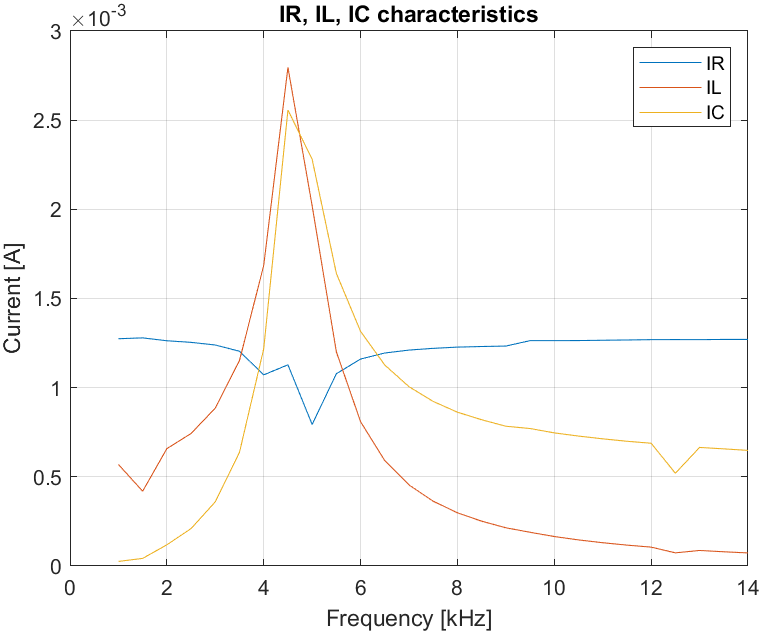
\includegraphics[width=0.7\textwidth]{Pictures/ct_char_05.png}
	\caption{$I_R$, $I_L$, $I_C$ characteristics graph}
	\label{fig:IR, IL, IC char}
\end{figure}

\subsubsection{Draw $U_R$, $U_{LC}$ characteristics as a function of frequency for rated parameters, assuming the value of supply voltage U = 5 V}

\subsubsection{Determine the goodness of the circuit for the resonant frequency from the knowledge of the currents}

\begin{equation}
    f_r=\frac{1}{2\pi\sqrt{LC}}=\frac{1}{2\pi\sqrt{22*10^{-3}*52*10^{-9}}}=4705.514537\approx4705\text{[Hz]}
\end{equation}

\begin{equation}
    Q=\frac{I_C}{I_R}=\frac{0.0026}{0.0011}=2.36
\end{equation}

\begin{equation}
    Q=\frac{I_L}{I_R}=\frac{0.0028}{0.0011}=2.54
\end{equation}
\subsubsection{Plot the characteristics of G, BL, BC, $|Y|$ as a function of frequency}

\begin{figure}[H]
	\centering
	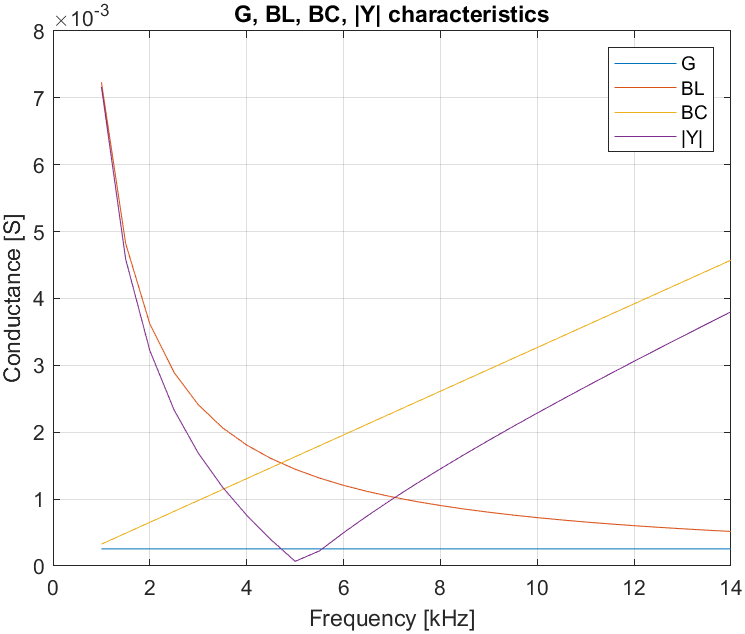
\includegraphics[width=0.7\textwidth]{Pictures/ct_char_06.png}
	\caption{G, $B_L$, $B_C$, $|Y|$, characteristics graph}
	\label{fig:G, BL, BC, Y char}
\end{figure}

\subsubsection{Determine from the given parameters:}

\begin{itemize}
    \item[a)]resonant pulsation
    \begin{equation}
        \omega_r=2\pi f_r\approx2\pi *4705\approx29562.38687\approx29560\text{[rad/s]}
    \end{equation}
\end{itemize}

\begin{itemize}
    \item[b)]resonant frequency
    \begin{equation}
        f_r=\frac{1}{2\pi\sqrt{LC}}=\frac{1}{2\pi\sqrt{22*10^{-3}*52*10^{-9}}}=4705.514537\approx4705\text{[Hz]}
    \end{equation}
\end{itemize}

\section{Conclusions and final comments}

\begin{flushleft}
    When the characteristic properties of series resonance circuit occurs the coil and capacitor behave like a short circuit. The impedance of the whole circuit is equal to resistance on resistor as it is showed on the graph with characteristics lines. Moreover the quality factor of the circuit is the biggest when the resonance is achieved.    
\end{flushleft}

\begin{flushleft}
    The results of occurring the resonance in parallel circuit is different than it was in series configuration because the coil and capacitor behaves like an open circuit. It is clearly showed in graph with the admittance characteristic line (the admittance is very small so the impedance is very big). 
\end{flushleft}

\end{document}